\section{System Modeling}
\phantomsection

% TODO refactor diagram captions

This chapter contains an attempt to model the application by use of UML
diagrams so that the further development of the system is easier and has well
defined boundaries. As a rule, the process of modeling an information system
usually starts off by laying out a general picture and then deepens into more
detailed views of the inner workings of the system.


\subsection{Use Case Layout of the Game}

Use case diagrams are used to provide a good understanding of what a user can
do with the application in question. In a nutshell, a game is out there to be
played and the 'Snowfight' is no exception. The gameplay has a rather simple
concept behind it and includes several things:

\begin{itemize}
	\item Moving around the field
	\item Throwing snowballs at adversaries
	\item Being eliminated from a game by being hit with snowballs
	\item Using the phone as a controller device
\end{itemize}

Besides playing the game itself, the players are able to view game results after
a match has finished and they can also modify the character's appearance and
name before the game starts.

\begin{figure}[!h]
\centering
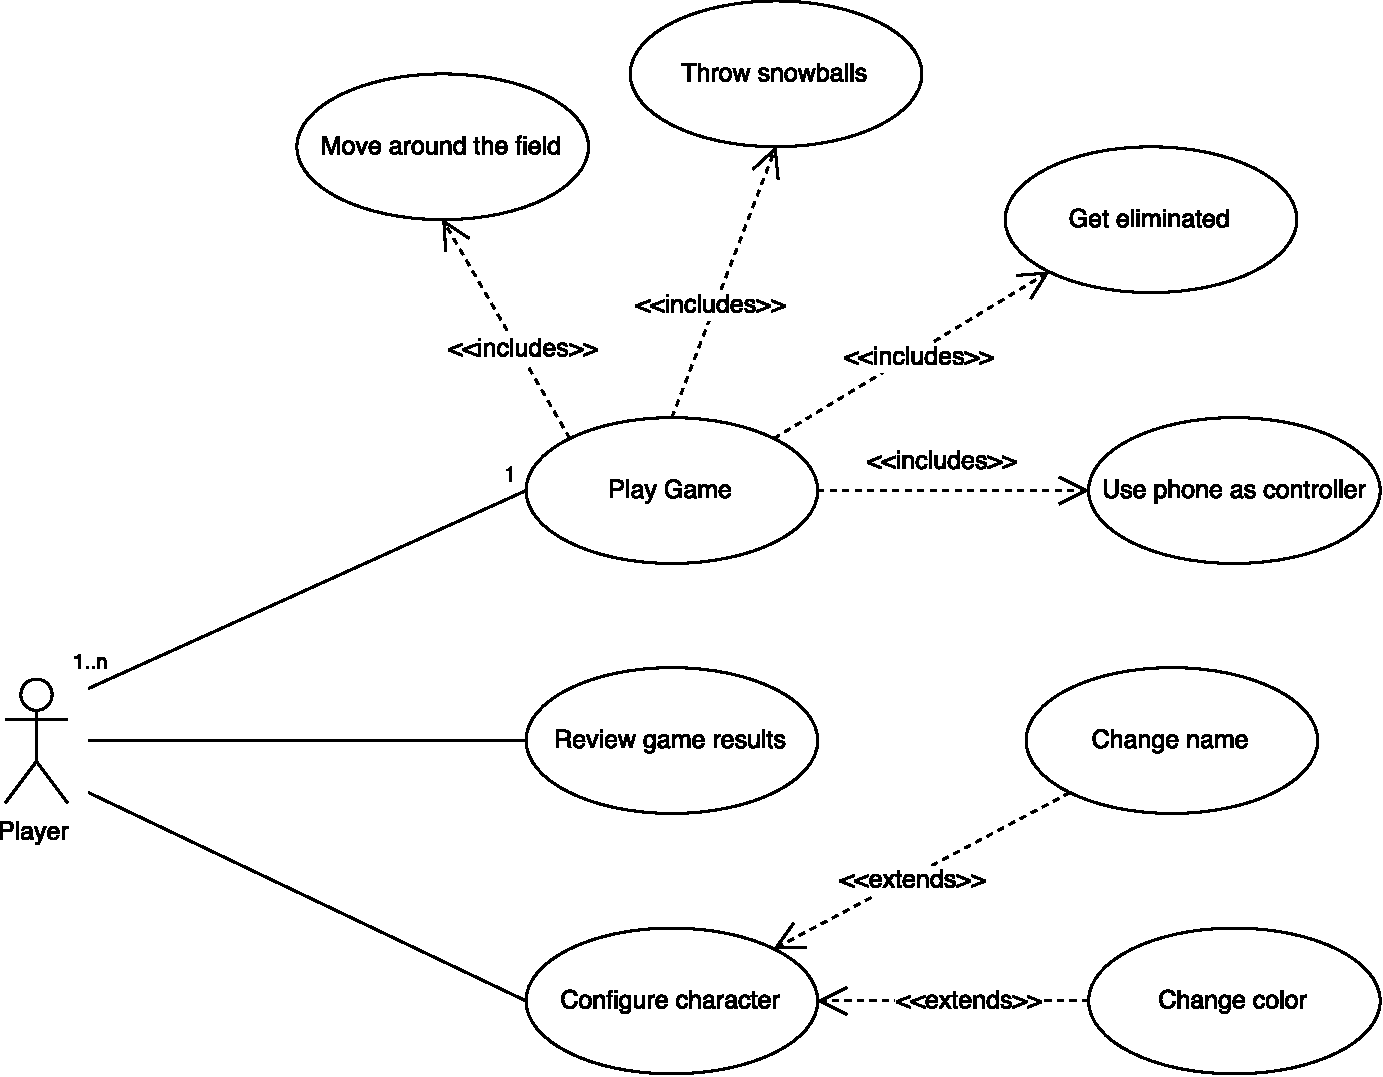
\includegraphics[width=15cm]{diagrams/usecase}
\caption{Game Use Cases from the Player's Perspective}\label{diag:usecase}
\end{figure}

\newpage

\subsection{User Activity Graph}

When it comes to the sequence of activities that may take place as part of the
use of an application, the activity diagram does an excellent job at
illustrating the transitions between different activities and various conditions
that might alter the activity flow.

A typical set of activities that take place as part of playing 'Snowfight' is
represented in the graph below. The players start off by accessing the index
page of the game in a web browser. This brings them in a game lobby that
contains a shareable URL used to connect controllers. Players navigate to this
URL in the browser on their smart-phones, personalize some character
configurations and connect to the game by pressing the start button on their
'controllers'. When all players are connected, the game is ready to start, which
is done by hitting the respective button in the game lobby. Now the players
enter the game loop, that is, they play a match, review the results and are
given the opportunity to restart the match and when all players make their
decisions the game is restarting leaving out those players who chose to quit.

\begin{figure}[!h]
\centering
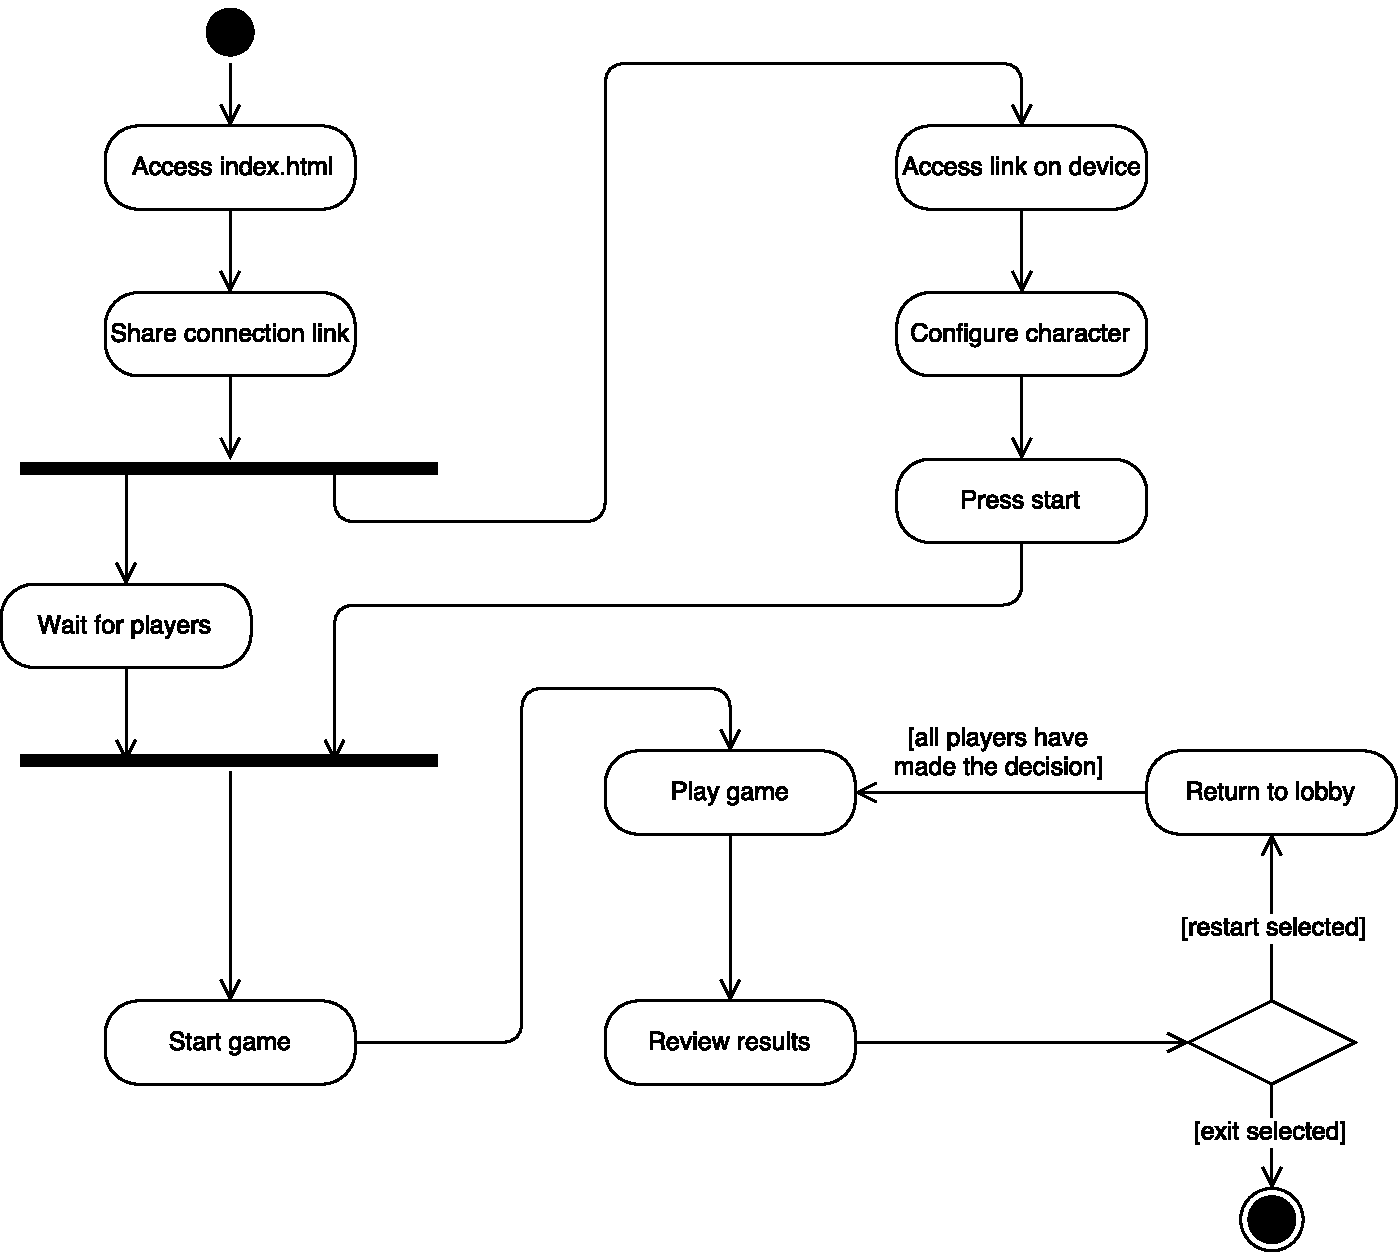
\includegraphics[width=15cm]{diagrams/activity}
\caption{Top-level Activities of the User}\label{diag:activity}
\end{figure}

\newpage

\subsection{High-level Game States}

When compared to simple web applications, games have a very substantial
distinction in the sense that they are real-time system. A web page can be
considered pretty much static once it has rendered, and all that happens
afterwards is the result of various event handlers modifying the obtained
document. Games, on the other hand, are being rendered to the screen every
fraction of a second and keep changing as a living system. All this takes place
in a, so called, game loop, and it is quite difficult to implement the various
stages the game passes through in a single chain of 'if's. This is why even at
the modeling stage, the game is split in different states through which it can
pass and which have different things to render and process.

The game in question has four main states:

\begin{description}
	\item [Lobby] - works like a simple web page and is used to gather players before game
	\item [Asset pre-loading] - is the period after the 'start' button was hit, but before the game simulation begins, and it is responsible for preparing all the assets before they are used
	\item [Active game] - the state in which the main gameplay takes place that performs all physics computations and rendering, it also includes the game logic
	\item [Results overview] - is like an interlude between matches, when the game simulation is stopped and only information about the match is rendered to the screen
\end{description}

\begin{figure}[!h]
\centering
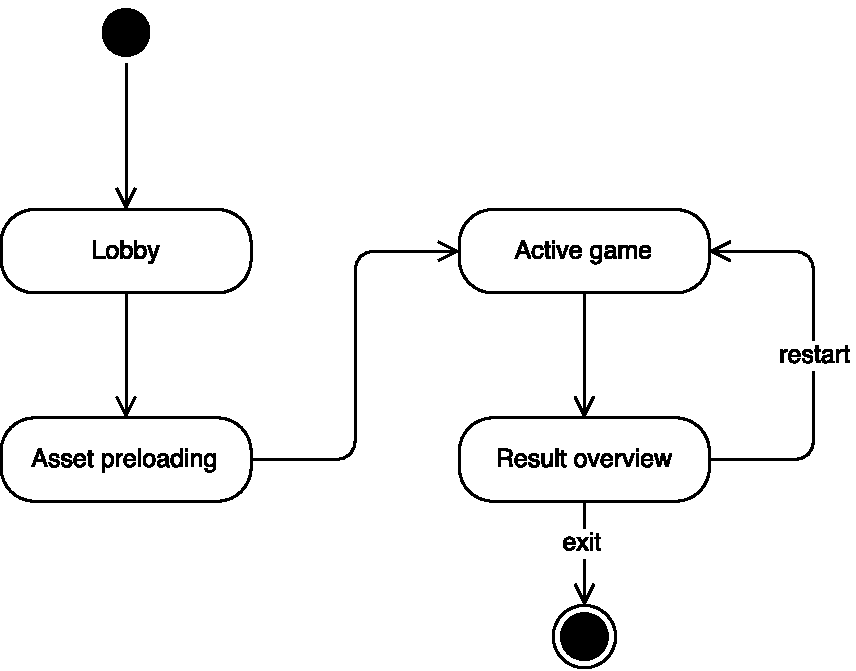
\includegraphics[width=15cm]{diagrams/state_2}
\caption{Game States}\label{diag:state_2}
\end{figure}

\newpage

\subsection{Player State Machine}

At a lower level the game logic is controlled by the states of individual game
objects and the main game object of the 'Snowfight' game is the player. It quite
convenient to model the player as a state machine because the way it is render,
the way it is updated and the manner in which it reacts to input heavily depend
on its current state. When put in real context, it becomes clear that it is not
possible to use the same animation or texture for a player that moves as well as
for a player that is disabled. In these two states the player also has different
kind of response to user input. When in default state, the player can move
around the field as a reaction to the motion controller, as opposed to the
situation of a disabled player when any kind of input has a null result.

\begin{figure}[!h]
\centering
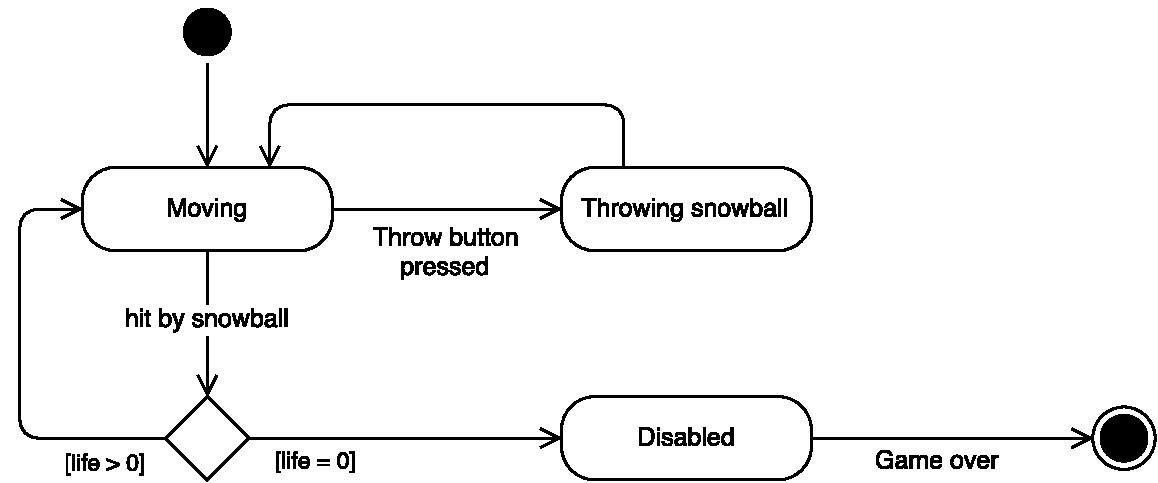
\includegraphics[width=\textwidth]{diagrams/state_1}
\caption{Player States}\label{diag:state_1}
\end{figure}

As it can be observed in the diagram above, the \emph{moving} state is the
default state as well as the first one in which the player starts the game. The
transition to another state might happen it two cases, and specifically, if the
user hits the button for throwing snowballs, the player transitions to the
respective state, the appropriate animation is played and the logic of trowing a
snowball is triggered. As soon as the \emph{throwing} process gets to its end,
the player transitions back to the \emph{moving} state automatically. In the
second case, the state change is set off by a game event rather than through
direct user input, that is, when a player is hit by a snowball of an adversary,
the state machine reaches a decision point. The amount of 'health points' of the
player in question is assessed and recalculated and if it is equal to zero, the
player enters the \emph{disabled} state and is considered eliminated from the
game till the end of the match, otherwise, an automatic transition back to the
\emph{moving} state takes place.

\newpage

\subsection{Class Hierarchy of Game Objects}

In the process of modeling a software system, an important role goes to laying
out the relationships between different classes of objects. Class diagrams are
recognized as one of the most effective tools that is able to convey a
comprehensive view of the structure of an information system. When it comes to
the game depicted in this thesis, the player is once again in the center of
attention as it is acts as a container for various game components and
represents the main logical unit of the game.

The diagram below illustrates the main classes defined in the project and the
relations between them. It can be observed that the Player class responds to
some standard methods that can be found in almost every game out there:
\emph{render}, \emph{update} and \emph{handleInput}. These methods are the
connection points of this object to the rest of the game and are invoked in the
respective sections of the game loop. Besides standard methods, a Player
contains helper methods like \emph{startMoving} and \emph{throwSnowball} that
would normally be invoked in the \emph{update} method, however, the state
machine architecture imposes a slightly different pattern. Instead of performing
all the logic in the methods mentioned above, the Player delegates the decisions
of 'what to do' to a state object that executes necessary actions depending on
the specific state of the Player. The states are managed by an object of
PlayerStateManager class, whose reference is stored in a field of a Player.

\begin{figure}[!h]
\centering
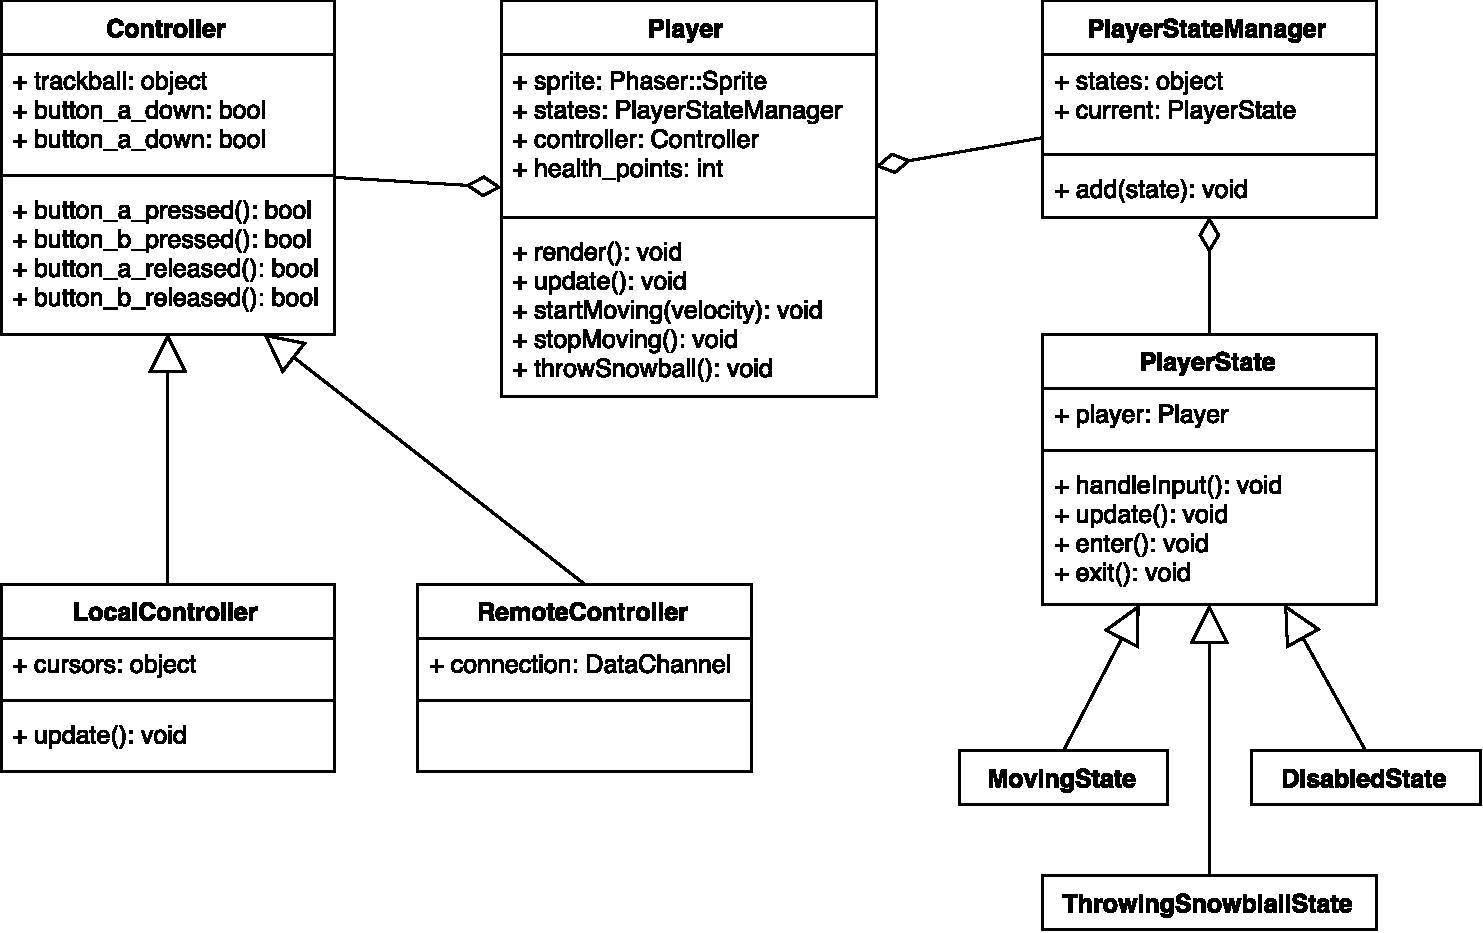
\includegraphics[width=15cm]{diagrams/class}
\caption{Player Class and Its Components}\label{diag:class}
\end{figure}

Another aspect of the architecture worth mentioning is the unified interface of
a controlling unit. The Player holds a reference to a Controller object, which,
in turn, can be of different types. This is motivated by the fact that the game
can be later modified to support artificial intelligence bots as adversaries at
the same time maintaining the same controller interface. Thus, a Player can
gather input information in the same way, regardless of the input source,
whether it is a local keyboard, a remote smart-phone or just a bot script.

\newpage

\subsection{Components and Libraries}

At the very beginning of the software development industry, programs had to be
written almost entirely from scratch, which took quite a bit of time and effort,
and usually it had to be redone with every following project. Today, however,
the vast majority of recurring problems have been solved and their programming
solutions can be found in various libraries that can be included and used in
independent projects. This way, software development has become biased from
writing all the code from zero, towards a more modular approach where
applications would share pieces of reusable software and the programmers would
only write code to glue all of it together.

Below is a component diagram that represents the dependency graph of the
'Snowfight' game. It points out what are the main components of the application
and which libraries are used to obtain the desirable functionality.

\begin{figure}[!h]
\centering
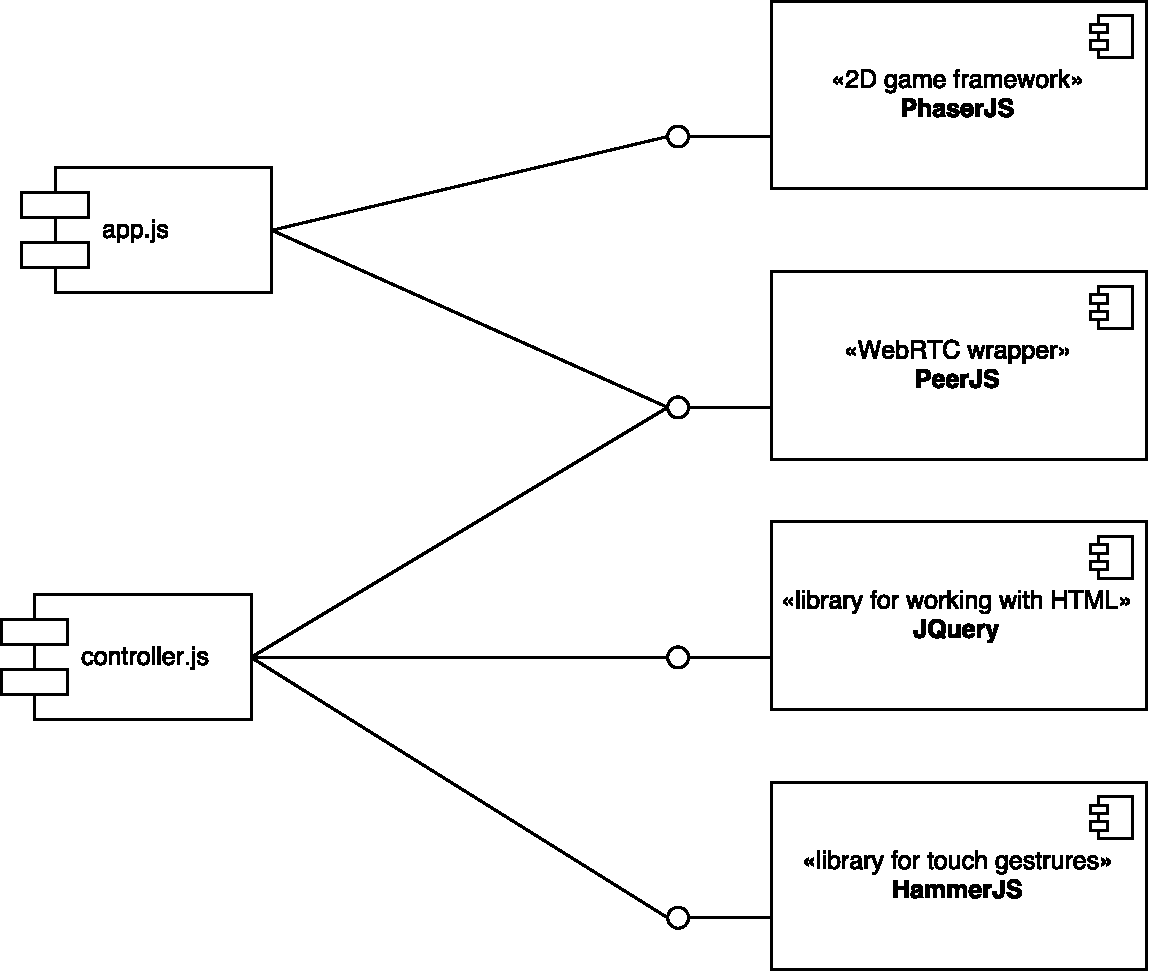
\includegraphics[width=15cm]{diagrams/component}
\caption{Component Diagram}\label{diag:component}
\end{figure}

The two components of the application are the main game module and the module of
the controller code. These modules share a dependency which is the 'PeerJS'
library. It is used to establish peer two peer connections between the game and
controllers, thus, it should be present in both places. The main game makes
extensive use of the PhaserJS game development library, while the controller
code exclusively includes a library for processing touch gestures called
HammerJS.

\newpage

\subsection{Deployment Setup}

When the application is moved to production it is important to understand the
deployment configuration of the system in order to be able to manage it
efficiently. In case of the game in question, it is not enough to consider only
a web server that would host the application files. The specifics of peer to
peer communication protocol involved in the project, require a dedicated service
for brokering the connections. In setups where raw WebRTC is used it is
necessary to deploy a STUN or TURN server. On the other hand, this project
includes a wrapper library that features a pre-configured server application.
This server application can be deployed in one of the three variants:

\begin{itemize}
	\item Hosted on the same machine as the web server
	\item Deployed to a separate dedicated server
	\item A third-party SaaS (Software as a Service) solution
\end{itemize}

The diagram that follows, illustrates the second type of deployment when the web
server and the 'PeerJS' server are hosted on two different dedicated machines.
The web server delivers the appropriate scripts to the client's devices. This
communication is performed using HTTP or HTTPS protocols. Client devices (a
computer and a phone), in turn, establish a peer-to-peer WebRTC connection, as a
result of communications with the broker server which are executed over a
combination of HTTP and WebSocket protocols.

\begin{figure}[!h]
\centering
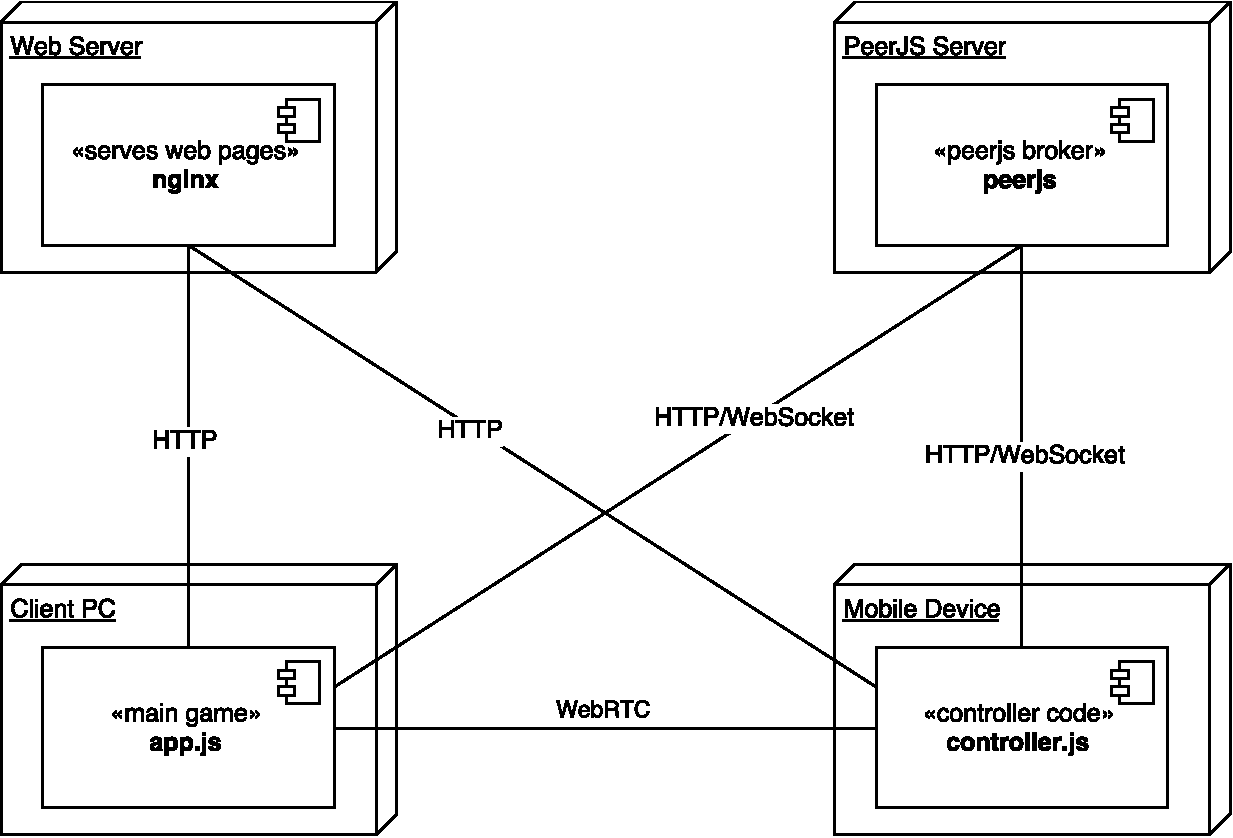
\includegraphics[width=15cm]{diagrams/deployment}
\caption{Deployment Diagram}\label{diag:deployment}
\end{figure}

\newpage

\subsection{System Design Conclusions}

This chapter provided an overview of the system design process of the
'Snowfight' game. By means of different types of UML diagrams it was possible to
obtain several perspectives of the most important parts of the application model
from different points of view.

It can be observed that the application design follows a couple of architectural
patterns found mostly in the game development industry, for example, the
stateful approach to modeling game objects. On the other hand, a lot of
particularities still can be traced back to the fact that the application is not
a native one, but rather web-based.

The value of system design can be hardly seen in such small projects as the one
depicted in this thesis, however, large systems cannot go without a good round
of design and analysis. Moreover, developer teams with a big number of employees
can vastly benefit from having diagrams that describe various parts of a system.
These provide documentation and make it easier for people who are new in the
project to pick up the material and continue further development.

\clearpage
